\documentclass[11pt, A4paper,norsk]{article}
\usepackage[utf8]{inputenc}
\usepackage[T1]{fontenc}
\usepackage{babel}
\usepackage{amsmath}
\usepackage{amsfonts}
\usepackage{amsthm}
\usepackage{amssymb}
\usepackage[colorlinks]{hyperref}
\usepackage{listings}
\usepackage{color}
\usepackage{hyperref}
\usepackage{graphicx}
\usepackage{cite}
\usepackage{textcomp}
\usepackage{float}

\definecolor{dkgreen}{rgb}{0,0.6,0}
\definecolor{gray}{rgb}{0.5,0.5,0.5}
\definecolor{daynineyellow}{rgb}{1.0,0.655,0.102}
\definecolor{url}{rgb}{0.1,0.1,0.4}

\lstset{frame=tb,
	language=Python,
	aboveskip=3mm,
	belowskip=3mm,
	showstringspaces=false,
	columns=flexible,
	basicstyle={\small\ttfamily},
	numbers=none,
	numberstyle=\tiny\color{gray},
	keywordstyle=\color{blue},
	commentstyle=\color{daynineyellow},
	stringstyle=\color{dkgreen},
	breaklines=true,
	breakatwhitespace=true,
	tabsize=3
}

\lstset{inputpath="C:/Users/Torstein/Documents/UiO/Fys2130/Python programmer"}
\graphicspath{{C:/Users/Torstein/Documents/UiO/Fys2130/"Python programmer"/}}
\hypersetup{colorlinks, urlcolor=url}

\author{Torstein Solheim Ølberg}
\title{Svar på Oblig nr. 6 i Fys2130}



%\lstinputlisting{Filnavn! type kodefil}
%\includegraphics[width=12.6cm,height=8cm]{Filnavn! type png}



\begin{document}
\maketitle
	\begin{center}
\Large \textbf{Oppgaver}
	\end{center}









		\paragraph{13.}
			\subparagraph{4)}
				\begin{flushleft}
Hvis spalten ikke har noe intensitets minimum kan vi si at spalten er større en bølgelengden $\lambda$ til lyset. Dette kan vi si ved hjelp av sammenhengen som står på siden $376$ i læreboka. Der står det at det første intensitetsminimummet har en vinkel $\theta$ fra midten, gitt ved
$$\sin(\theta) = \frac{\lambda}{a}$$
der $a$ er bredden på spalten. Dette betyr at $\sin(\theta)$ må være større enn $1$ og da må spalten ha en bredde større enn $\lambda$.
				\end{flushleft}








		\paragraph{15.}
			\subparagraph{5)}
				\begin{flushleft}
Hvis de to stripene er veldig langt fra hverandre vil vinkelen mellom hver av maksimaene være veldig veldig små, og det vil være vanskelig å se forskjell på de forskjellige maksimaene og minimaene. Er derimot spaltene veldig nærme hverandre vil det være så stor vinkel mellom maksimaene at det til slutt kanskje bare er ett maksima. I begge disse to tilfellene vil det se ut som det bare er en tykk stripe på midten, akkurat som hvis det hadde vært partikler og ikke bølger som ble sendt avgårde. \\
Når det gjelder denne oppgaven så er det veldig vanskelig å si noe, siden det er helt umulig å si om disse spaltene er spesielt nærme eller langt fra hverandre.
				\end{flushleft}









			\subparagraph{6)}
				\begin{flushleft}
Hvis det bare trenger å være en sammenheng mellom bølgene i ett spesifikt punkt kan denne sammenhengen være med større og større avstand i tid. Hvis denne avstanden i tid går mot uendelig er bølgene ikke-koherente, så det er en gradvis overgang mellom koherente og ikke-koherente bølger jo nærmere uendelig tid det er mellom hvert "event" skjer.
				\end{flushleft}

			








		\paragraph{13}
			\subparagraph{11)}
				\begin{flushleft}
Vinkelen mellom andre og tredje intensitets minima er gitt ved:
$$\theta_{3} - \theta_{2} = \arcsin\left( \frac{\lambda}{d} \left( \frac{5}{2} \right) \right) - \arcsin\left( \frac{\lambda}{d} \left( \frac{3}{2} \right) \right)$$
$$\theta_{3} - \theta_{2} = \arcsin\left( \frac{5 \cdot 500 \text{nm}}{2 \cdot 0.450 \text{mm}} \right) - \arcsin\left( \frac{3 \cdot 500 \text{nm}}{2 \cdot 0.450 \text{mm}} \right)$$
$$\theta_{3} - \theta_{2} = \arcsin\left( \frac{2.500}{900} \right) - \arcsin\left( \frac{1.500}{900} \right)$$
$$\theta_{3} - \theta_{2} = \arcsin\left( 0.00278 \right) - \arcsin\left( 0.00167 \right) \approx 0.00278 - 0.00167 = 0.00111$$
Siden det er mye mye større avstand mellom skjermen og spaltene, enn det er mellom spaltene selv, kan vi se på en trekant mellom midten spaltene og de to midtpunktene for intensitetsminimummene. Denne trekantene vil ha to rettvinklede vinkler ved de to mørke linjene, og den siste vinkelen er $0.00111$. Da er avstanden mellom de to linjene tilnærmet lik
$$7.5 \text{m} \cdot  \sin(0.00111) = 0.0833 \text{m}$$
				\end{flushleft}










			\subparagraph{13)}
				\begin{flushleft}
Putter du et stykke glass foran en av spaltene vil bølgen som treffer denne spalten komme inn fra en annen retning enn bølgen som treffer den andre spalten. Det eneste dette vil gjøre er at interferensmønsteret vil bli forskjøvet littegran i den retningen hvor spalten med glass er.
				\end{flushleft}










			\subparagraph{17)}
				\begin{flushleft}
Ser jeg på håret som en dobbelspalte. Antar at hvert av de to mørke områdene ligger på hver sin side av midten på skjermen. Hvis det er $185 \text{cm}$ mellom håret og skjermen, og det er $8.1 \text{cm}$ mellom midten på skjermen og et av de mørke områdene. Det betyr at det er en vinkel $\theta$ mellom linja fra hårstrået til midten av skjermen og linja fra håret til det mørke området, er gitt ved $\arcsin\left( \frac{185}{8.1} \right) = 0.04380$. Hvis vi antar at diameteren til hårstrået er mye mye mindre enn $185 \text{cm}$ kan vi bruke at $d = \frac{\lambda}{\sin(\theta)} \left( n + \frac{1}{2} \right)$, hvor $n$ er nummeret til det mørke området, altså $6$ i vårt tilfelle.
$$d = \frac{532 \text{nm}}{\sin(0.04380)} \left( 6 + \frac{1}{2} \right) = \frac{532 \text{nm}}{\sin(0.04380)} \frac{13}{2} = \frac{6916 \text{nm}}{0.08757} = 78970 \text{nm}$$
$$d = 78.97 \text{$\mu$m}$$
På nettet fant jeg at et hår kan ligge mellom $17$ og $181$ mikrometer, ut i fra hvilken kilde jeg vil bruke, som passer ganske bra med utregningen min.
				\end{flushleft}









			\subparagraph{19)}
				\begin{flushleft}
En CD fungerer slik at når du lyser med en laser på cden vil laseren bli reflektert i en spesifikk vinkel når det treffer en rille. Antar at det er meningen at dette skal fungere som en spalte når lyset blir reflektert. Da vil lyset bli reflektert til vinklene
$$\theta = \arcsin\left( \frac{n \cdot 632.8 \text{nm}}{1600 \text{nm}} \right) = \arcsin\left( n \cdot 0.3955 \right)$$
				\end{flushleft}











		\paragraph{15.}
			\subparagraph{15)} $ $
				\begin{figure}[H]
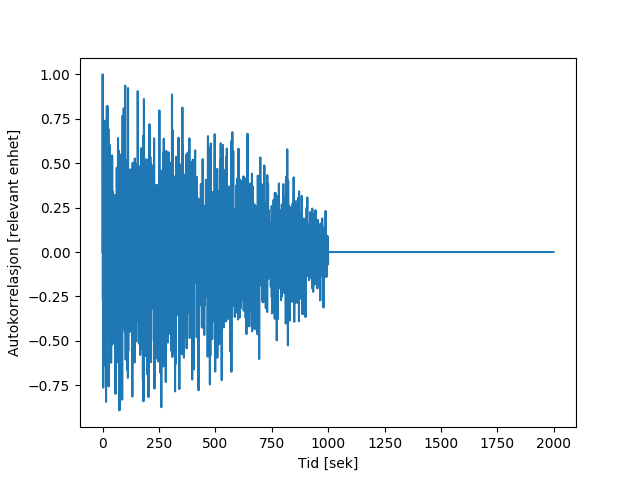
\includegraphics[width=12.6cm, height=9cm]{Figur_0008.png}
\caption{Plott av autokorrelasjonen til en funksjon med senterfrekvens $5000$ og fullbredde frekvens $3000$.}
				\end{figure}
				\begin{flushleft}
Ut i fra dette plottet ser det ut til at koherenstiden ligger rundt $750 \text{sek}$. Føler ikke jeg har noen spesiell utgangspunkt for å si noe om dette, men siden eksemplene i boka ligger på rundt $2 \text{ms}$ ville jeg trodd at det skulle være ganske mye kortere tid.
				\end{flushleft}
\lstinputlisting{Oblig6_15_15.py}











			\subparagraph{16)} $ $
				\begin{figure}[H]
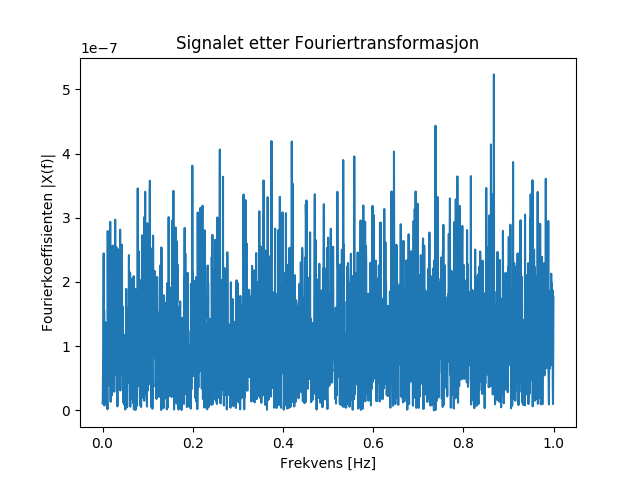
\includegraphics[width=12.6cm, height=7.7cm]{Figur_0009.png}
\caption{Fourertransformasjon av signalet}
				\end{figure}
				\begin{figure}[H]
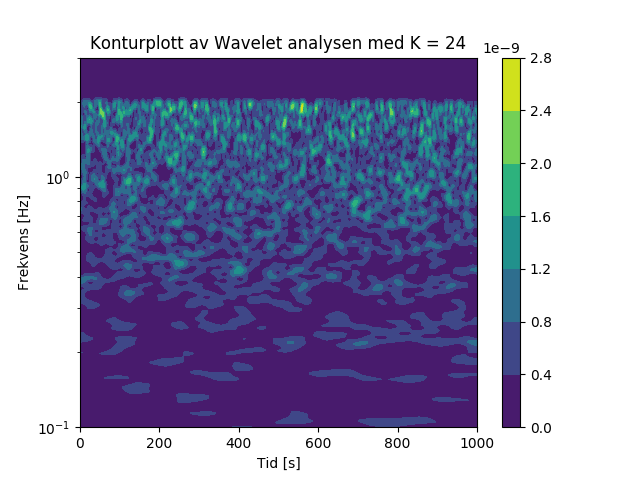
\includegraphics[width=12.6cm, height=7.7cm]{Figur_0010.png}
\caption{Wavletanalyse av signalet}
				\end{figure}
				\begin{figure}[H]
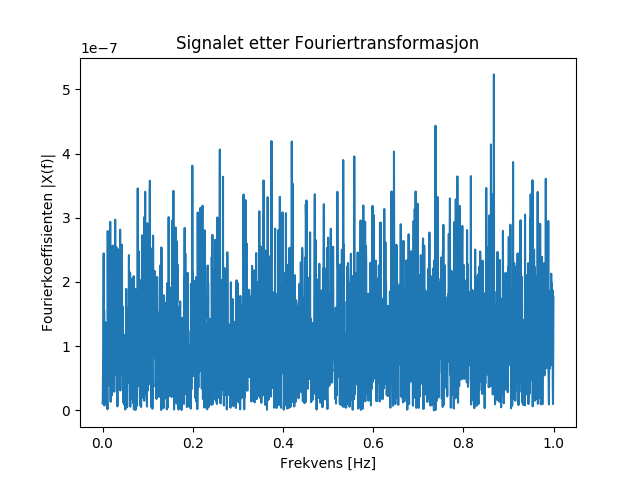
\includegraphics[width=12.6cm, height=7.7cm]{Figur_0011.png}
\caption{Fouriertransformasjon av signalet kvadrert}
				\end{figure}
				\begin{figure}[H]
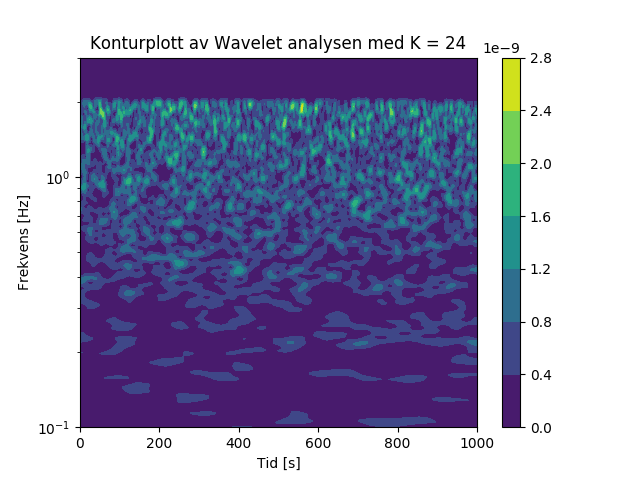
\includegraphics[width=12.6cm, height=7.7cm]{Figur_0012.png}
\caption{Wavletanalyse av det kvadrerte signalet}
				\end{figure}
				\begin{flushleft}
Alle disse bildene viser at signalene vi har består av stort sett alle forskjellige frekvenser mellom $0.1$ og $2$, men hovedsaklig fra $1$ og opp til $2$. Da jeg prøvde å sjekke alle frekvensene fra $0.1$ og opp til $8000$ fikk jeg an hel masse striper over alt, men dette virka veldig usannsynlig at skulle være riktig, for prøvde jeg å sette $K$ høyere så fikk jeg bare en ensfarget firkant. Øker jeg $K$ for dette bildet får jeg bare at det er en masse spesifikke streker over alt.
				\end{flushleft}
\lstinputlisting{Oblig6_15_16.py}
\end{document}